\chapter{Martedì 09/03/2021}
\section{Iniziamo ad uccidere il compilatore}
\begin{itemize}
	\item Il file .o è un file di sistema che non dipende dal linguaggio compilato: posso partire da files .s, .cpp, .c...
	\begin{center}
		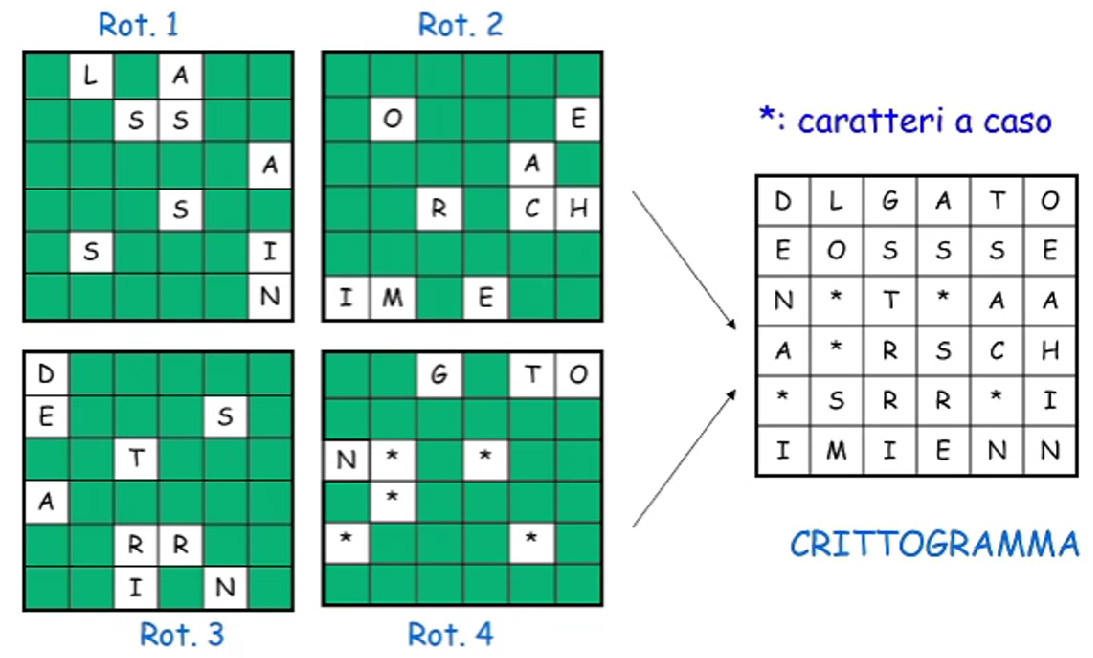
\includegraphics[scale=0.90]{img/12.PNG}
	\end{center} 
	\item Abbiamo due opzioni:
	\begin{itemize}
		\item scrivere un file in c o in c++, per esempio, passandolo da un compilatore che restituirà un file assembler;
		\item scrivere direttamente del codice assembler evitando il compilatore.
	\end{itemize}
	\item I comandi gcc e g++ non sono veri e propri compilatori, ma dei \emph{front-end}: capiscono quali strumenti devono utilizzare, e in che ordine, per ottenere l'eseguibile  finale.
\end{itemize}
\clearpage

\subsection{Esercizio dai lucidi del prof.Frosini} 
\paragraph{Testo}Vogliamo realizzare un programma diviso in due parti:
\begin{itemize}
	\item la prima col programma principale
	\item la seconda col sottoprogramma \emph{esamina}, usato dal primo file.
\end{itemize}
Il programma
\begin{itemize}
	\item legge caratteri fino al fine linea;
	\item per ogni carattere, oltre a stamparlo, chiama il sottoprogramma \emph{esamina}, e stampa il risultato prodotto da quest'ultimo.
\end{itemize}
Il sottoprogramma esamina restituisce otto caratteri in codifica ASCII, corrispondenti agli 8 bit della codifica del carattere ricevuto.

\small
\begin{multicols}{2}
	\paragraph{Codice di esamina.s}
	\begin{verbatim}
		.global esamina, alpha, beta
		
		.data
		alpha:  .byte 0
		.align 8  
		beta:   .quad 0
		
		.text
		esamina:
		push %rax
		push %rdx
		push %rcx
		
		mov alpha(%rip), %cl
		movabs beta, %rax
		mov $0, %rdx
		prossimo:
		test $0b10000000, %cl
		jz zero
		
		movb $'1', (%rax, %rdx)
		jmp avanti
		zero:
		movb $'0', (%rax, %rdx)
		jmp avanti
		avanti:
		shl %cl
		inc %rdx
		cmp $8, %rdx
		jb prossimo
		
		pop %rcx
		pop %rdx
		pop %rax
		ret
	\end{verbatim}
	\paragraph{Codice di codifica.s}
	\begin{verbatim}
		.include "ser.s"
		.global _start
		
		.data
		buffer:
		.fill 8,1
		
		.text
		_start:
		call tastiera
		cmp $'\n', %al
		je fine
		call video
		mov %al, alpha
		lea buffer, %rax
		mov %rax, beta(%rip)
		call esamina
		mov $' ', %al
		call video
		mov $0, %rcx
		ancora:
		mov buffer(,%rcx), %al
		call video 
		inc %rcx
		cmp $8, %rcx
		jb ancora
		
		mov $'\n', %al
		call video
		jmp _start
		fine:
		call uscita
	\end{verbatim}
\end{multicols}
\normalsize
\paragraph{Riflessioni}
\begin{itemize}
	\item \textbf{Trasmissione dei dati fra programma e sottoprogramma}. Dobbiamo utilizzare due variabili \emph{alfa} e \emph{beta} definite nel secondo file (\emph{extern} nel primo e \emph{global} nel secondo). La prima contiene il codice del carattere che il sottoprogramma deve esaminare, la seconda contiene l'indirizzo di una variabile array di 8 byte, dove il sottoprogramma deve porre il risultato. Il programma principale pone i dati in \emph{alfa} e \emph{beta}, quindi chiama \emph{esamina}.
	\item Abbiamo utilizzato una libreria contenuta nel file \emph{ser.s}. Per il momento il contenuto di questi sottoprogrammi non ci interessa (ne riparleremo più avanti).
	\item \textbf{Direttive \emph{global}}. Nel file \emph{esamina.s} le variabili \emph{alfa} e \emph{beta} sono dichiarate globali dalla seguente direttiva
	\begin{verbatim}
		.global esamina, alpha, beta
	\end{verbatim}
	se non facciamo questo l'altro file non potrà usare queste etichette. Ricordarsi che il collegatore vede solo ciò che è \emph{global}.
	\item \textbf{Reminiscenza di Reti logiche}. La PUSH e la POP devono essere utilizzate in modo adeguato (eseguo le push all'inizio del sottoprogramma, le pop alla fine del programma, inoltre per determinare l'ordine delle istruzioni POP considero l'ordine delle PUSH).
	\begin{verbatim}
		push %rax
		push %rdx
		push %rcx
		
		[...]
		
		pop %rcx
		pop %rdx
		pop %rax
		ret
	\end{verbatim}
	\begin{itemize}
		\item \textbf{Cosa succede se non eseguo le istruzioni pop alla fine?} L'istruzione RET alla fine del sottoprogramma \emph{esamina} prende l'indirizzo che sta in cima alla pila: il problema è che abbiamo eseguito la push altre tre volte dopo la chiamata del sottoprogramma, quindi l'elemento in cima alla pila non è quello che dovrebbe usare la RET. Se l'indirizzo considerato (quello che si cerca di trattare come indirizzo) ci porta a un'area non assegnata al programma otterremo l'errore di \emph{segmentation fault}.
		\item \textbf{Cosa succede se poniamo le POP in ordine non consueto?} I registri non vengono riportati al loro valore originario. L'errore non viene segnalato, ma può provocare risultati indesiderati.
	\end{itemize}
	\item \textbf{Sintassi per gli indirizzi}. Attenzione alla rip
	\begin{verbatim}
		mov alpha(%rip), %cl
	\end{verbatim}
	Siamo certi che questo indirizzamento ci permette di evitare problemi. La cosa non è necessaria in questo caso: il programma è molto piccolo.
	\item \textbf{Istruzione \emph{test} in \emph{esamina.s}}. L'istruzione
	\begin{verbatim}test $0b10000000, %cl\end{verbatim}
		equivale all'istruzione AND, ma non viene modificato il destinatario. L'unica cosa modificata sono i flag. 
		\item \textbf{Sostituzione automatica della \emph{mov} con la \emph{movabs}}. Se poniamo qualcosa che non è rappresentabile su 32 bit
		\begin{verbatim}
			mov $0x12345668, %rax
		\end{verbatim}
		l'assemblatore adotta automaticamente la movabs (il destinatario è un registro, nient'altro). Provare per credere!
		\begin{framed}
			\item \textbf{Azzeramento della parte alta di un registro a 64 bit}. Se il registro è a 32 bit la parte alta viene sempre azzerata (\underline{novità}). Segue che le seguenti istruzioni\begin{verbatim}
				mov $0, %edx
				mov $0, %rdx
			\end{verbatim}
			avranno lo stesso effetto
		\end{framed}
		\item \textbf{Natura dell'operando destinatario} (banalità importante). Possiamo scrivere...? \begin{verbatim}cmp %rdx, $8\end{verbatim} 
			No: la destinazione è per natura un registro o un indirizzo in memoria (sempre, anche se l'istruzione non ci scrive) 
			\item \textbf{Domanda da pretest di Reti logiche}. Cosa fa la seguente istruzione..?
			\begin{verbatim}
				mov $beta, %rax
			\end{verbatim}
			La stessa cosa della LEA: pone come contenuto del registro rax l'indirizzo relativo all'etichetta \emph{beta}. Possiamo fare la stessa cosa così:
			\begin{verbatim}lea beta, %rax\end{verbatim}
				\item \textbf{Allineamento e disallineamento}. Attenzione ai dati
				\begin{verbatim}
					.data
					alpha:  .byte 0
					beta:   .quad 0
				\end{verbatim}
				Sono disallineati: \emph{alpha} si trova all'offset 0, \emph{beta} all'offset 1. Segue che un byte di \emph{beta} si troverà in un'altra regione naturale (dunque sono necessari due accessi). L'assemblatore non interviene, a meno che non poniamo la seguente direttiva
				\begin{verbatim}
					.data
					alpha:  .byte 0
					.align 8
					beta:   .quad 0
				\end{verbatim}
				La direttiva mi permette \emph{di scartare i prossimi elementi in modo tale da arrivare al prossimo multiplo di 8}.
				\begin{center}
					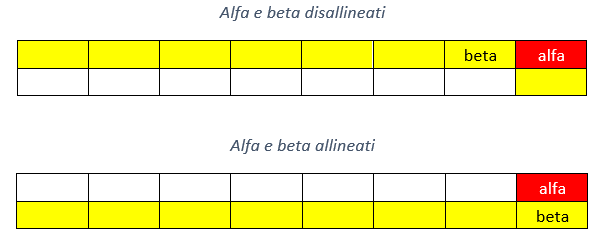
\includegraphics[scale=.85]{img/149.PNG}
				\end{center} 
				\item \textbf{Etichette esterne}. L'assemblatore per default assume che tutte le etichette non definite in un file siano \emph{esterne}, cioè definite in un file esterno. Possiamo indicarlo in modo esplicito con una direttiva
				\begin{verbatim}
					.extern alpha
				\end{verbatim}
				Il linker, che ha visione completa (in contrasto all'assemblatore), inchioda se si accorge che certe etichette non sono state definite.
				\begin{itemize}
					\item \textbf{Cosa succede se non uso global per segnalare ad altri files ulteriori etichette?} Si segnala errore di \emph{undefined reference} dopo aver avviato il linker. L'etichetta è definita (si veda \emph{nm}), ma non viene vista nell'altro file.
					\item \textbf{Cosa succede se dichiaro un'etichetta beta globale in esamina.s e ne introduco una con lo stesso nome in codifica.s?} Se un file presenta un'etichetta con un certo nome e questa viene usata nel file stesso non c'è motivo per andarla a cercare altrove. \underline{Quella che avviene è una \emph{sovrapposizione} rispetto alla variabile} \underline{globale dichiarata altrove}.
				\end{itemize}
			\end{itemize}
			
			\chapter{Giovedì 11/03/2021}
			\section{Programmi misti C++/Assembler}
			Oggi vogliamo cominciare a scrivere programmi misti, cioè scritti in parte in C++ (passati dal compilatore) e in parte in Assembler. 
			
			\subsection{g++ e \emph{startfiles}} Il g++ è un front-end per i vari strumenti preconfigurato per programmi scritti in C++. Capisce cosa deve fare e chiama opportunamente compilatore e/o assemblatore (in base ai files che gli passiamo)
			\begin{verbatim}
				g++ -o nome_file_output -no-pie file1, file2, ...
			\end{verbatim}
			creiamo un eseguibile con nome \emph{codifica} a partire dai files indicati nel comando. Il parametro \emph{-no-pie} viene posto per evitare degli errori (non approfondiremo il perché).  
			\paragraph{Proviamolo} Proviamo ad eseguire g++ con il programma scritto durante la scorsa lezione 
			\begin{verbatim}
				g++ -o codifica -no-pie codifica.s esamina.s
			\end{verbatim}
			creiamo un eseguibile con nome \emph{codifica} a partire dai file \emph{codifica.s}, \emph{esamina.s}. Il terminale ci segnala errore:
			\begin{center}
				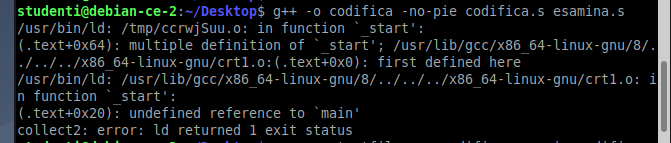
\includegraphics[scale=.9]{img/150.PNG}
			\end{center} 
			\paragraph{Come mai?} g++ aggiunge, senza dire nulla, degli \emph{start files} che fanno delle inizializzazioni (fatte prima della partenza del programma vero e proprio): in questi file oggetto aggiuntivi viene definito \emph{$\_$start}, che fa un po' di cose e chiama, alla fine, la funzione \emph{$\_$main}. Possiamo evitare questi inserimenti ponendo un ulteriore parametro nell'istruzione
			\begin{verbatim}
				g++ .nostartfiles -o codifica -no-pie codifica.s esamina.s
			\end{verbatim}
			Se facciamo questa cosa col problema visto nella scorsa lezione tutto funziona regolarmente. Non avendo utilizzato cose non nostre non ci sono problemi nell'ignorare gli \emph{startfiles}.
			\paragraph{Cosa potrebbe fare la start?}
			\begin{itemize}
				\item Definire strutture e classi (se io dichiaro un'istanza globale di una classe dovrò avere già definita la classe al momento dell'esecuzione di main)
				\item Inizializzazione di oggetti cin e cout (che, va be, sono classi)
				\item Esecuzione dei distruttori
			\end{itemize}
			\paragraph{Standard C++}  Definiamo \emph{main} invece di \emph{start} e poniamo RET alla fine del programma. Abbiamo una chiamata del sottoprogramma main all'interno di start: dopo che main ha restituito il controllo la start esegue quanto necessario per concludere l'esecuzione del programma, incluso i distruttori.
			\subsection{g++ e \emph{overloading}}
			\paragraph{Scriviamo l'analogo in C++ di codifica.s}
			\begin{verbatim}
				#include <iostream>
				
				extern char alpha; 
				extern char* beta;
				extern void esamina();
				
				char buffer[8];
				
				int main() {
					while(true) {
						char c;
						std::cin.get(c);
						
						if(c == `\n')
						break;
						
						alpha = c; <--- devo dire al compilatore chi e' alpha          [LO FACCIO SOPRA]
						beta = buffer; <--- devo dire al compilatore chi e' beta
						
						esamina(); <-- devo dire al compilatore chi e' esamina
						for(int i = 0; i < 8; i++) {
							std::cout << buffer[i];
						}
						std::cout << "\n";
					}
				}
			\end{verbatim}
			\clearpage
			\noindent Se eseguiamo il codice
			\begin{verbatim}
				g++ -no-pie -o codifica1 codifica1.cpp esamina.s
			\end{verbatim}
			si lamenta perché non trova \emph{esamina}. 
			\begin{center}
				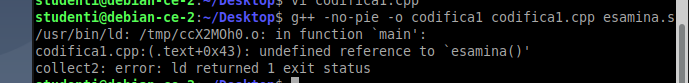
\includegraphics{img/151.PNG}
			\end{center} 
			Vediamo cosa succede controllando gli elementi definiti in codifica1.cpp
			\begin{verbatim}
				g++ -c codifica1.cpp <---- mi limito ai files oggetto
				nm codifica1.o <---- leggo simboli definiti
			\end{verbatim}
			\begin{center}
				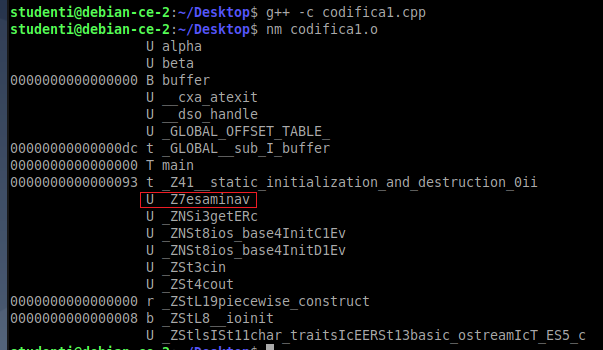
\includegraphics{img/152.PNG}
			\end{center} 
			troviamo esamina, ma con un nome strano.
			\paragraph{Causa} Il compilatore storicamente ha sempre usato gli stessi collegatori del C. Sappiamo che differenza sostanziale tra C e C++ è la presenza dell'overloading nel secondo (cioè funzioni con nome uguale e parametri diversi). Nel nostro caso l'etichetta per esamina è la seguente
			\begin{verbatim}
				_Z7esaminav
			\end{verbatim}
			$\_$Z è un prefisso obbligatorio, 7 è il numero di caratteri del nome della funzione, v significa void (cioè assenza di parametri). Non possiamo gestire più funzioni con lo stesso nome mediante le stesse etichette, dobbiamo differenziarle! 
			\paragraph{Soluzione}
			\begin{itemize}
				\item O modifico l'extern ponendo quel nome strano (vedremo più avanti le convenzione relative ai nomi delle etichette in C++)
				\begin{verbatim}
					extern void _Z7esaminav();
				\end{verbatim}
				\item O pongo l'extern nel seguente modo
				\begin{verbatim}
					extern "C" void esamina();
				\end{verbatim}
				esiste \emph{una funzione esamina che non ha argomenti, posta in un altro file, e scritta in C} (ok, non è scritta in C, ma rispetta lo standard del C). Nel C non esiste l'overloading, quindi le etichette assumono il nome che ci aspettiamo.
			\end{itemize}
			Chiaramente non serve questa cosa per le altre extern: non esiste l'overloading per le variabili.
			\paragraph{Analogo in C++ di esamina.s}
			\begin{verbatim}
				char alpha;
				char* beta;
				
				extern "C" void esamina() { <-- extern serve solo per poter indicare "C", 
					<-- altrimenti abbiamo il problema di prima
					char c = alpha;
					for(int i = 0; i < 8; i++) {
						if(c & 0x80) {
							beta[i] = `1';
						}
						else {
							beta[i] = `0';
						}
						c << 1;
					}
				}
			\end{verbatim}
			
			\paragraph{E se volessimo solo l'assembler?} Poniamo l'istruzione così
			\begin{verbatim}
				g++ -fno-PIC -S codifica1.cpp <-- genero l'assembler
				vi codifica1.s <---- apro l'assembler
			\end{verbatim}
			Il codice ottenuto presenta le istruzioni Assembler che ci aspettiamo, più delle righe di codice contenenti principalmente informazioni (utili, per esempio, al debugger).
			
			\clearpage \subsection{Uso dei registri} 
			Vogliamo trovare un compromesso tra funzione chiamante e funzione chiamata: in particolare, vogliamo garantire al chiamante un certo numero di registri.
			
			\begin{center}
				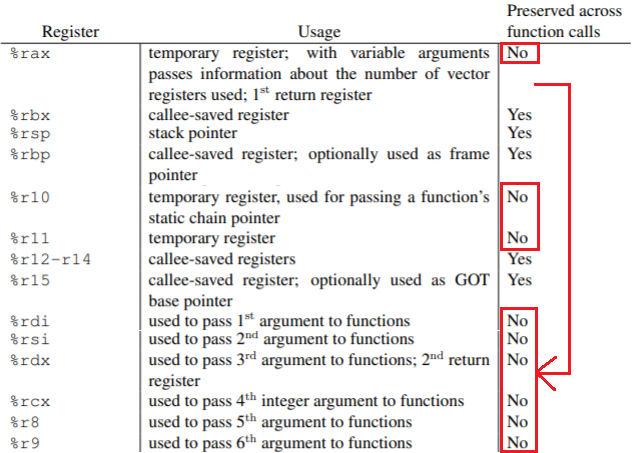
\includegraphics{img/269.PNG}
			\end{center} 
			\begin{itemize}
				\begin{framed}
					\item Alcuni registri sono detti \emph{scratch}, cioè possono essere usati liberamente dalla funzione chiamata senza dover salvare il contenuto pre-esistente:
					\begin{itemize}
						\item RAX, R10, R11, \underline{RCX, RDX, RSI, RDI, R8, R9} {\small (Per ricordare: A,C,D,S,8,9,10,11)}.
					\end{itemize}
					\item I registri rimanenti sono registri \emph{non scratch}, garantiti al chiamante (quindi non vengono toccati dalla funzione chiamata): RBP, RBX, R12, R13, R14, R15. 
				\end{framed}
				\item \textbf{Conseguenza}: dobbiamo stare attenti, il contenuto dei registri scratch non viene mantenuto in caso di chiamate di funzione. Noi dobbiamo preoccuparci esclusivamente dei nostri contenuti, dunque ricorrere alle istruzioni PUSH e POP se non vogliamo perdere il valore di alcuni registri scratch a seguito di chiamata di funzione.
			\end{itemize}
			\clearpage 
			
			\subsection{Rappresentazione dei dati}
			La cosa è molto intuitiva, ma c'è uno standard da eseguire. 
			\subsubsection{Tipi fondamentali} 
			Sono disponibili molte informazioni su \url{cppreference.com} alla voce \emph{Fundamental types}.
			\begin{center}
				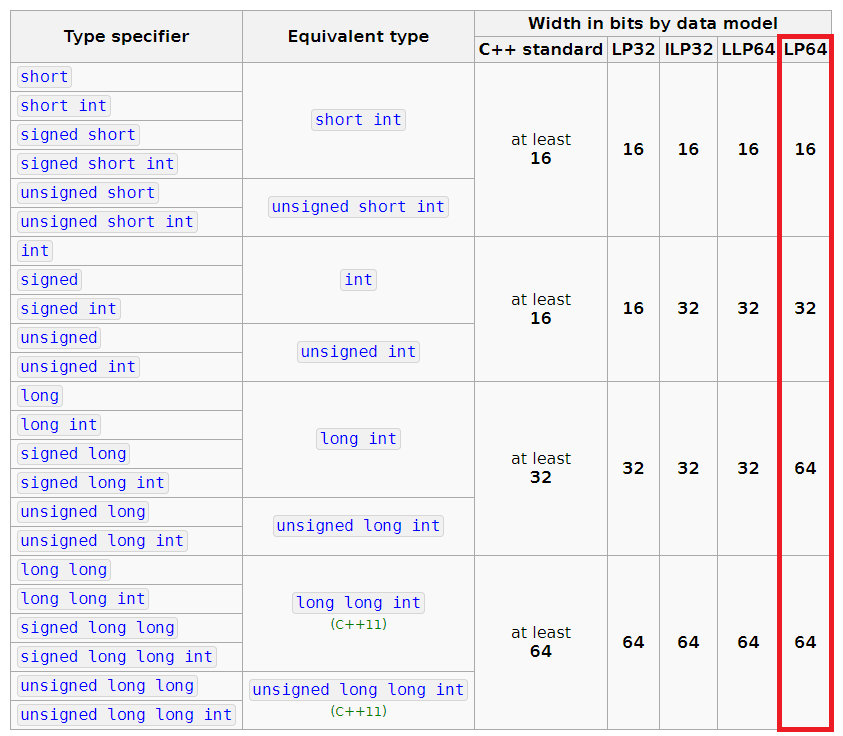
\includegraphics[scale=0.90]{img/13.PNG}
			\end{center} 
			Il sito mette insieme standard e implementazione: in particolare si osserva che lo standard da margini di liberta all'implementatore (si parla di \emph{almeno}, non un numero ben preciso). Questo significa che altri documenti dovranno specificare per intero come avviene l'implementazione. Sono riportate alcune implementazioni comuni nello standard. In particolare ci interessano LLP64 ed LP64: la prima è per windows, la seconda per i sistemi Unix e Unix-like (Linux, macOs).
			\clearpage 
			
			\paragraph{char} Cosa strana è la presenza di tre tipi diversi:
			\begin{itemize}
				\item \begin{verbatim}
					signed char
				\end{verbatim}
				tipica rappresentazione dei char in x86, x64.
				\item \begin{verbatim}
					unsigned char
				\end{verbatim}
				\item \begin{verbatim}
					char
				\end{verbatim}
				la rappresentazione sarà equivalente a signed char o unsigned char, ma rimane un tipo diverso.
			\end{itemize}
			\paragraph{Approfondiamo l'implementazione} Il documento che specifica tutto ciò che lo standard non dice (in Linux) è il \emph{System V Application Binary Interface}. Per quanto riguarda la rappresentazione dei dati abbiamo una tabella con tipi, dimensioni e allineamento. Caratteristica dei tipi fondamentali è avere dimensione e allineamento uguali.
			\begin{center}
				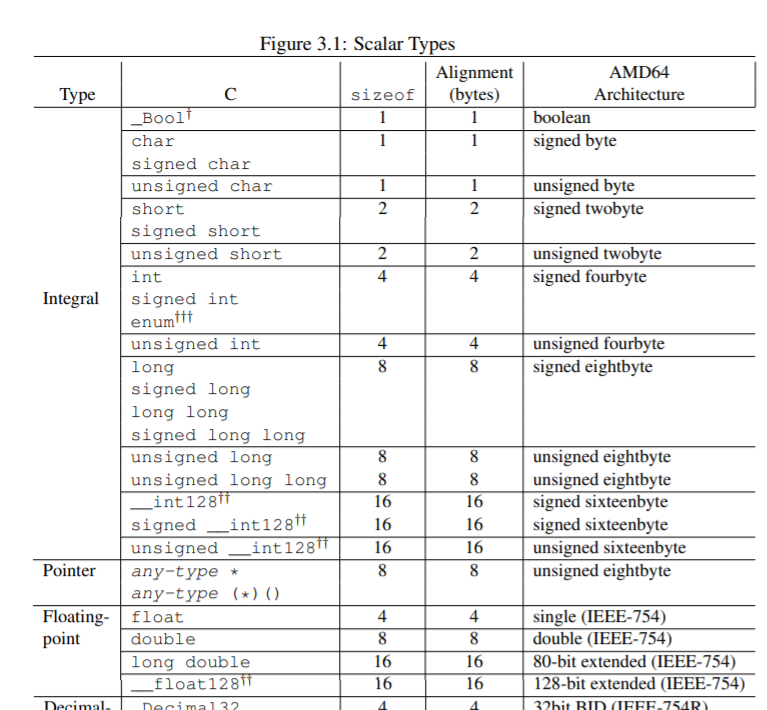
\includegraphics[scale=0.85]{img/14.PNG}
			\end{center} 
			\clearpage 
			
			\subsubsection{Tipi derivati}
			Quale dimensione e allineamento avranno i tipi derivati?
			\begin{itemize}
				\item \textbf{Puntatori}: hanno dimensione fissa al di la di cosa puntano, quindi valgono le cose già viste nella pagina precedente.
				\item  \textbf{Array}: \begin{verbatim}
					tipo a[DIM]
				\end{verbatim}
				\begin{multicols}{2}
					\begin{itemize}
						\item \emph{sizeof}: $\text{DIM} * \text{sizeof}(\text{tipo})$
						\item \emph{alignof}: $\text{alignof}(\text{tipo})$
					\end{itemize}
				\end{multicols}
				%\begin{center}
				%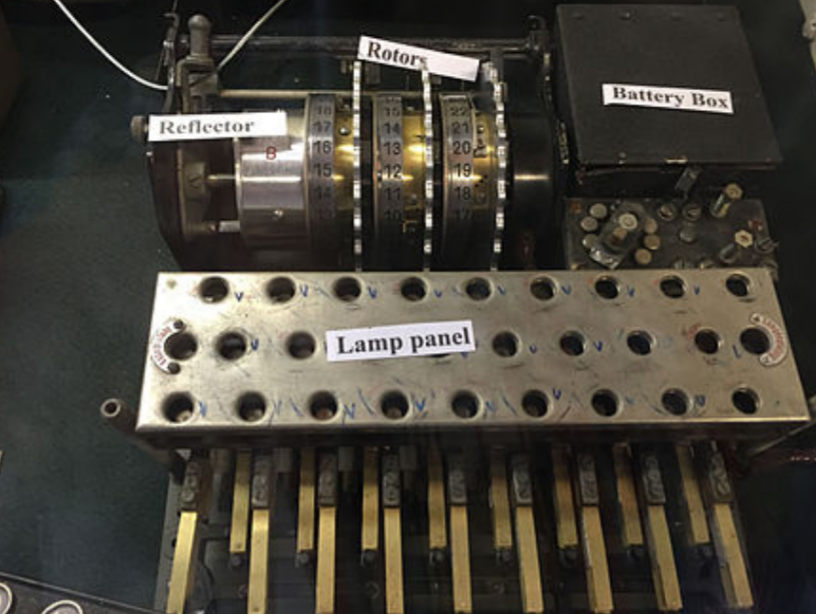
\includegraphics[scale=0.75]{img/15.PNG}
				%\end{center} 
				gli indirizzi crescenti, che partono da zero, mi rendono facile il calcolo dell'indirizzo di ogni elemento dell'array.
				
				\item \textbf{Strutture}: la cosa è un tantino più complicata.
				
				\begin{verbatim}
					struct s {
						tipo_1 f_1;
						tipo_2 f_2;
						tipo_3 f_3;
					}
				\end{verbatim}
			\begin{itemize}
					\item \emph{alignof}: \[\max_i\, \{ \text{alignof}(\text{tipo$_i$})\}\]
					\item \emph{sizeof}: non esiste una formula vera e propria, per prima cosa dobbiamo immaginarci il \emph{layout} della struttura. Consideriamo che:
					\begin{itemize}
						\item ogni elemento della struttura deve rispettare il proprio allineamento; 
						\item i campi devono trovarsi in memoria \textbf{nell'ordine in cui sono dichiarati} (non esistono forme di ottimizzazione in cui viene alterato l'ordine degli elementi);
						\item la dimensione totale della struttura deve essere un multiplo dell'allineamento della struttura.
					\end{itemize}
				\end{itemize}
			\end{itemize}
			\subsubsection{Primo esempio di struttura}
			\begin{center}
				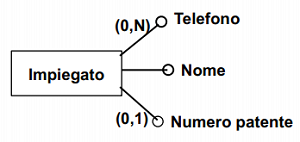
\includegraphics[scale=0.80]{img/16.PNG}
			\end{center} 
			\begin{itemize}
				\item Gli interi hanno dimensione $4$ e allineamento $4$. L'ordine in cui sono stati posti mi permette di porre i due interi nella stessa regione naturale. Il long ha dimensione $8$ e allineamento $8$. Dobbiamo allocarlo al primo indirizzo, multiplo di 8, successivo. 
				\item \textbf{Conclusioni}:\begin{itemize}
					\item \emph{alignof}: il massimo degli allineamenti è $8$.
					\item \emph{sizeof}: $16$ byte
				\end{itemize}
			\end{itemize}
			%\begin{itemize}
			%\item Contrariamente all'assemblatore il compilatore vuole conoscere tutte le etichette esistenti. Dobbiamo indicarlo noi con \emph{extern}.
			%\end{itemize}
			\subsubsection{Secondo esempio di struttura}
			\begin{center}
				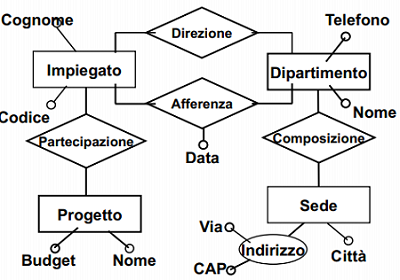
\includegraphics[scale=0.80]{img/17.PNG}
			\end{center} 
			\begin{itemize}
				\item Contrariamente a prima non possiamo mettere il char assieme a un altro elemento: nè con long (che ha dimensione di 8 byte), nè con char (che si trova dopo long). L'allineamento è stringente e impone che il long sia posto in un indirizzo multiplo di 8. Seguono 7 byte inutilizzati nella regione dove si trova il primo char.
				\item Dopo long mettiamo l'altro char, che non pone particolari vincoli. Rimangono 7 byte (che non faranno parte della struttura).
				\item \textbf{Conclusioni}:\begin{itemize}
					\item \emph{alignof}: $8$ (il massimo tra gli alignof, il più alto è quello di long)
					\item \emph{sizeof}: $17$ byte, più $7$ byte non utilizzati.
				\end{itemize}
			\end{itemize}
			
			\paragraph{perché non si può ottimizzare l'ordine degli elementi?} Il compilatore non può ottimizzare l'ordine degli elementi per conto suo. 
			\begin{itemize}
				\item Supponiamo di avere due files distinti. Il compilatore lavora distintamente su questi due. 
				\item Se la struttura dipendesse dalle ottimizzazioni i due files potrebbero aver adottato ottimizzazioni diverse, quindi le due strutture non risulterebbero equivalenti.
				\item Se nei due files ci sono funzioni che comunicano tra di loro e che devono scambiarsi una struttura allora i due files devono concordare sul \emph{layout} della struttura.
			\end{itemize}
			
			\subsubsection{Terzo esempio di struttura}
			Prendiamo il seguente esempio
			\begin{center}
				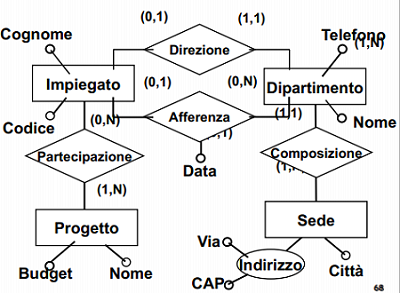
\includegraphics[scale=0.80]{img/18.PNG}
			\end{center} 
			L'unica cosa che conta è l'ordine degli elementi. Si consideri che l'allineamento di ogni singolo char di $s$ è $1$, quindi l'allineamento della struttura $s$ è $1$. Possiamo porre i byte di $s$ subito, senza passare subito a una nuova regione (niente ce lo vieta).